\chapter{The \lhcb detector}
\label{sec:Detector}
The Large Hadron Collider (LHC) of the European Organization for Nuclear Research CERN in Geneva, Switzerland is currently the world's most powerful particle accelerator.
Having a circumference of 26.7 \km it is designed to either collide protons with a centre-of-mass energy of $\sqs=14\tev$ or heavy ions with 2.8 \tev per nucleon \cite{LHC}.
The beams can be brought to collision at four interaction points.
At these points different experiments are placed.
Whereas \atlas and \cms are built as multi-purpose detectors \cite{ATLAS, CMS} and \alice studies heavy-ion collisions \cite{ALICE}, \lhcb is dedicated to search indirectly for evidence of physics beyond the Standard Model by the study of hadrons containing either a heavy \bquark- or \cquark-quark.

Those \B- and \D-hadrons are mainly produced by gluon-gluon fusion at \lhc energies with subsequent hadronisation.
These gluons in general carry different momenta leading to a boost of the hadron along the beam-pipe.
This is why the \lhcb detector is built as a single-arm forward spectrometer.
Its layout can be seen in figure \ref{fig:detector}.
\begin{figure}[hptb]
    \centering
	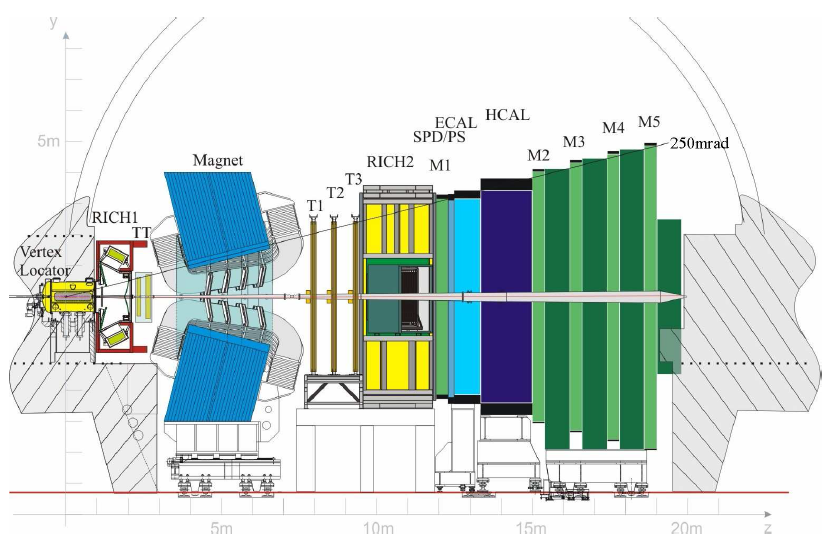
\includegraphics[width=\textwidth]{lhcb-detector}	
	\caption{The \lhcb detector.}
	\label{fig:detector}
\end{figure}
It has a forward angular coverage from approximately 10\mrad to 300\mrad in the bending respectively to 250\mrad in the non-bending plane.
A right-handed coordinate system is adopted with the $z$ axis along the beam-pipe and the $y$ axis pointing upwards along the vertical.
With this choice approximately 25\% of all \bquark\bquarkbar pairs are produced in the acceptance of the \lhcb detector \cite{bb_Production} though it covers only 4\% of the solid angle as shown in Figure \ref{fig:bb_Production}.
\begin{figure}[hptb]
    \centering
	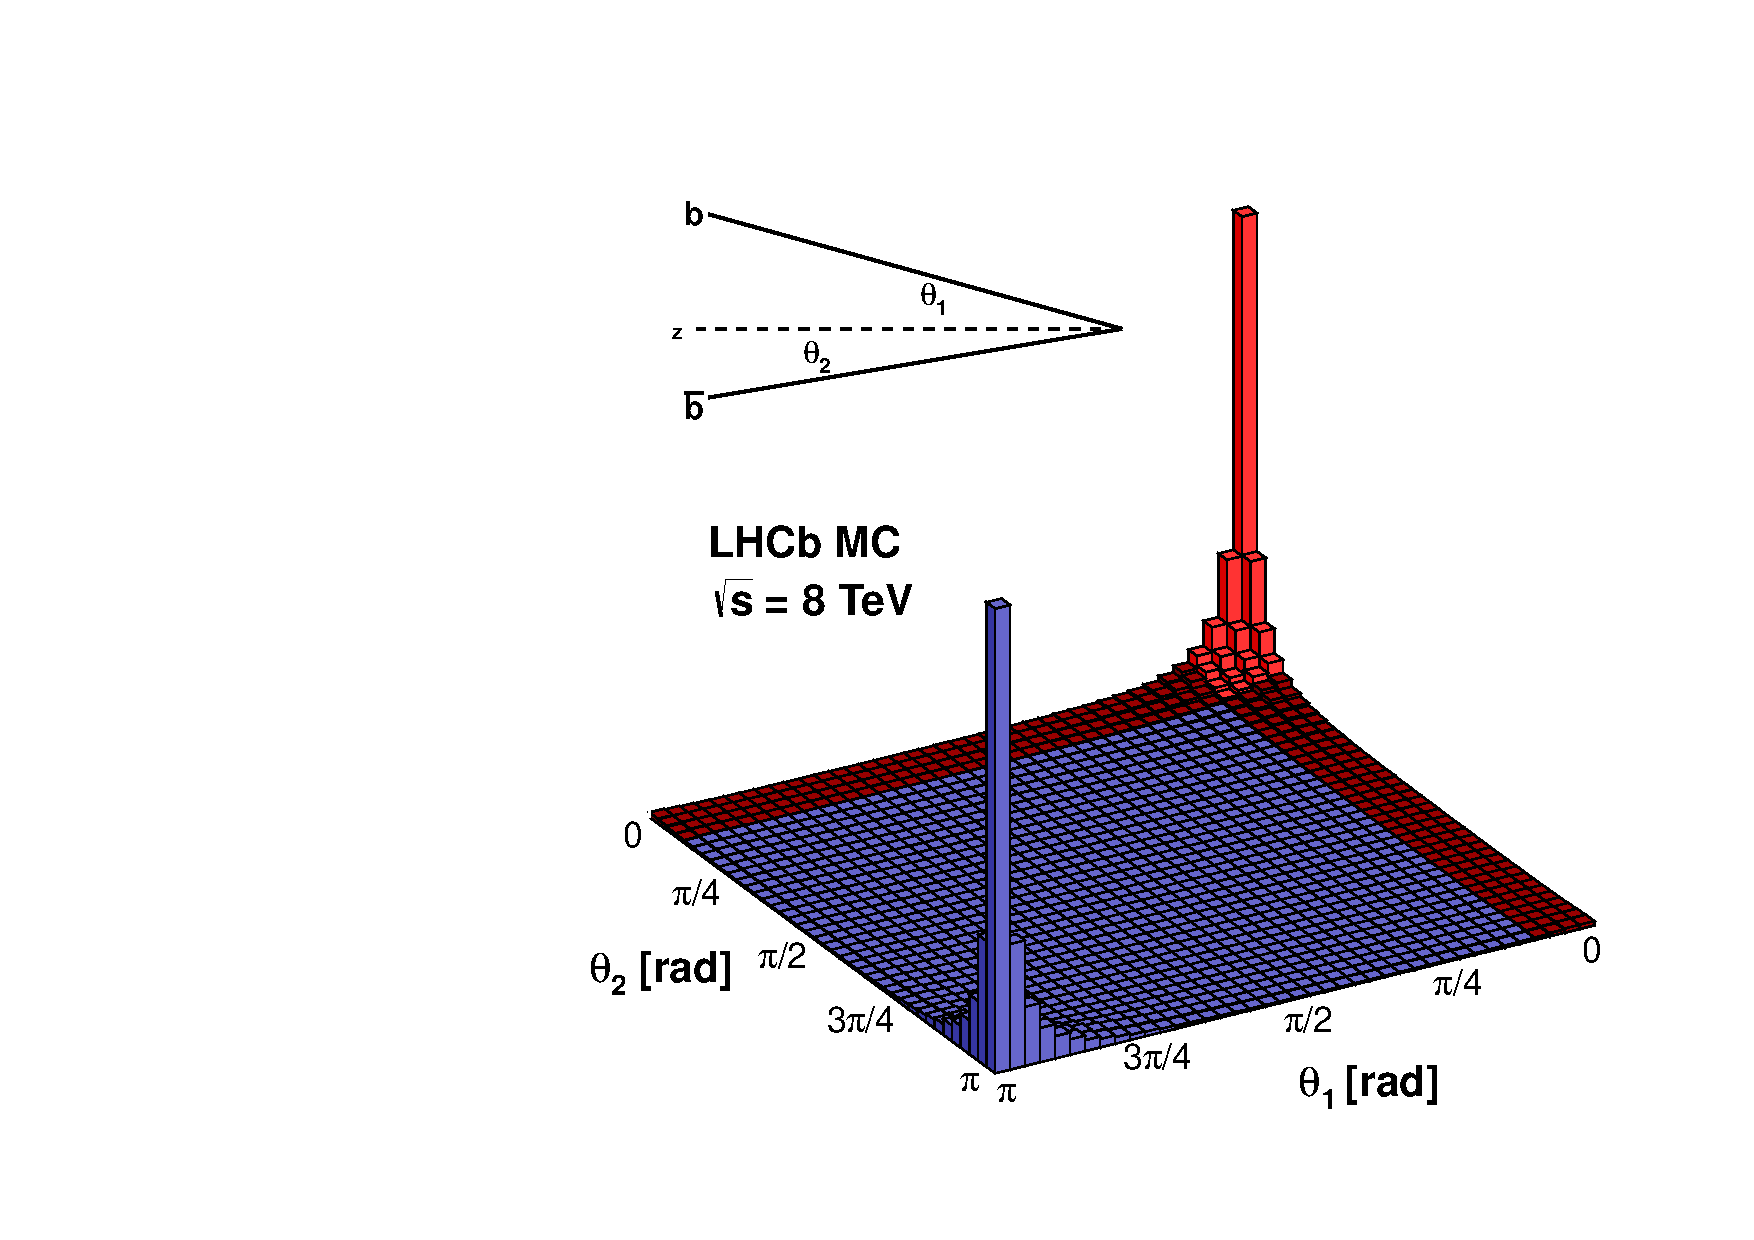
\includegraphics[width=0.5\textwidth]{bb_production}	
	\label{fig:bb_Production}
    \caption{Simulation of the \bquark\bquarkbar production in \proton\proton collisions at $\protect\sqs = 8 \protect\tev$.
             The angular acceptance of the \lhcb detector is coloured in red. Figure taken from.}
\end{figure}
The \lhcb detector consists of multiple subdetectors and sensors.
They can be roughly separated into two groups by their dedicated purpose.
They are in priciple either used for the reconstruction of particle tracks or to identify the particles.
Both groups will be explained in the following.

% ===========================
% SECTION: Tracking detectors
% ===========================
\section{Tracking detectors}
Tracking describes the whole procedure to reconstruct the trajectories of (charged) particles produced in the proton-proton collision. 
If there is a magnet in use, the particles' charges and momenta can be determined as well by the deflection of the track. 
For that purpose, a system of several subdetectors is aligned up- and downstream the dipole magnet, namely the Vertex locator (VELO), the Trigger Tracker (TT) and the Trigger stations (T1-T3) built-up by the Inner Tracker (IT) and the Outer Tracker (OT).

\subsection{Vertex Locator (VELO)}
The VErtex LOcator (VELO) is placed directly around the primary interaction point. 
Its task is to precisely measure the track coordinates of charged particles and separate the proton-proton interaction point from other vertices, namely either other primary vertices (so called pile-up events) or secondary vertices. 
The latter ones are typically for \bquark- or \cquark-hadron decays \cite{VELO_TDR} and a good separation and resolution of these vertices is crucial for the \lhcb physics programme.
As an example serves the measurement of particles' decay length and time for the determination of the rapid $\Bs-\Bsb$ oscillation frequency \cite{BsBsbar_frequency}.

The VELO is built up by silicon modules due to the high particle flux and thus high radiation in the interaction region. 
It is placed only 7\mm apart from the beam. 
This is closer than the required aperture of the \lhcb beam pipe at injection. 
Thus, the VELO sensors are made of silicon microstrips shaped as slightly overlapping half-discs. 
The two halfs can be moved in $x$- and $y$-direction to avoid radiation damages unless the beam is stable.

Each module provides a measurement of the $r$- and $\phi$-coordinates.
The sensores for these measurements are correspondingly called $R$- and $\Phi$-sensor, which can be seen in figure \ref{fig:VELO_RandPhiSensor}.
An overview over the VELO system with its modules is shown in figure \ref{fig:VELO_Overview}. 
Around the nominal interaction region, the modules are placed closer to each other. 
Upstream there are two $R$ sensors dedicated to veto pile-up events. 
Figure \ref{fig:VELO_Overview} furthermore shows the VELO in closed and opened position.
\begin{figure}[hptb]
    \centering
	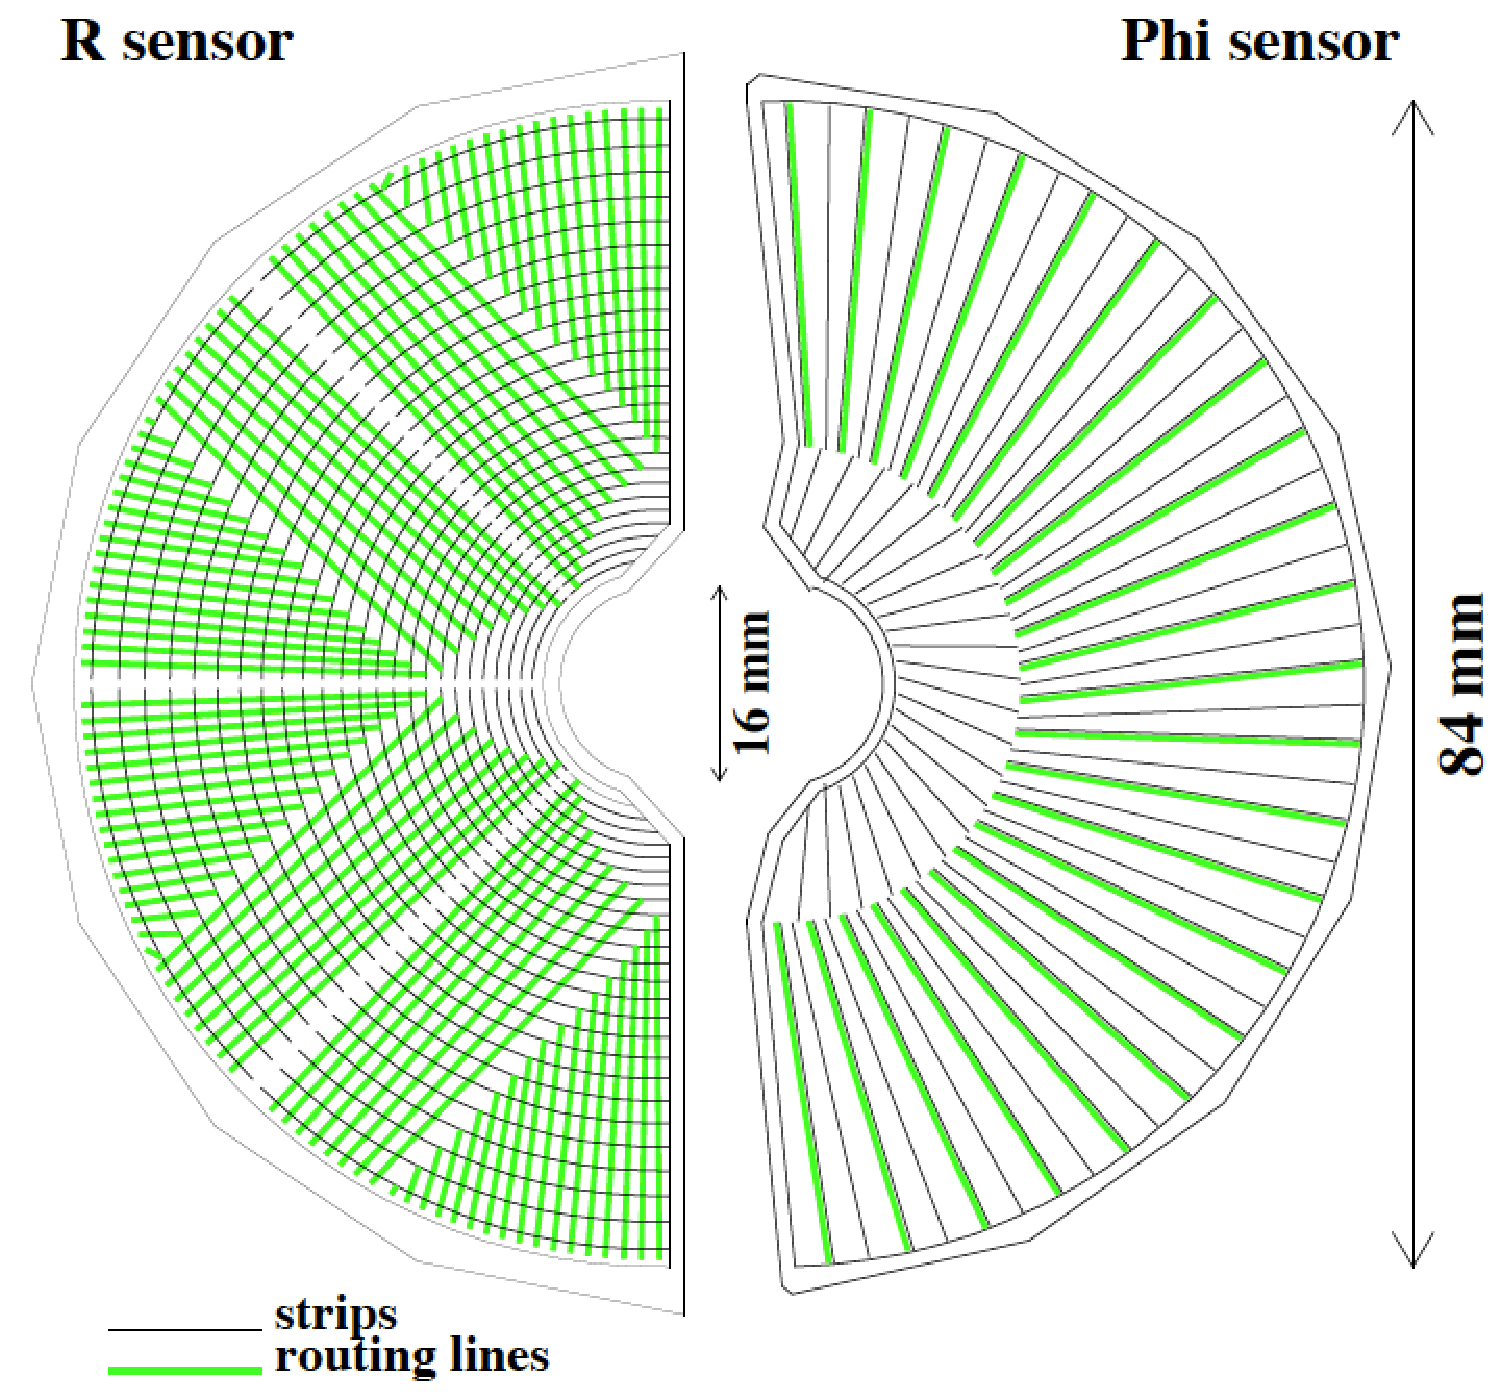
\includegraphics[width=0.5\textwidth]{VELO_randphisensors}	
	\caption{Schematic representation of an $R$ and a $\Phi$ sensor. The $R$ sensor strips are arranged into four approximately 45\degrees segments and have routing lines perpendicular to the strips. The $\Phi$ sensor has two zones with inner and outer strips. The routing lines of the inner strips
    are orientated parallel to the outer strips. Figure and caption taken from \cite{VELO_Performance}.}
	\label{fig:VELO_RandPhiSensor}
\end{figure}
\begin{figure}[hptb]
    \centering
	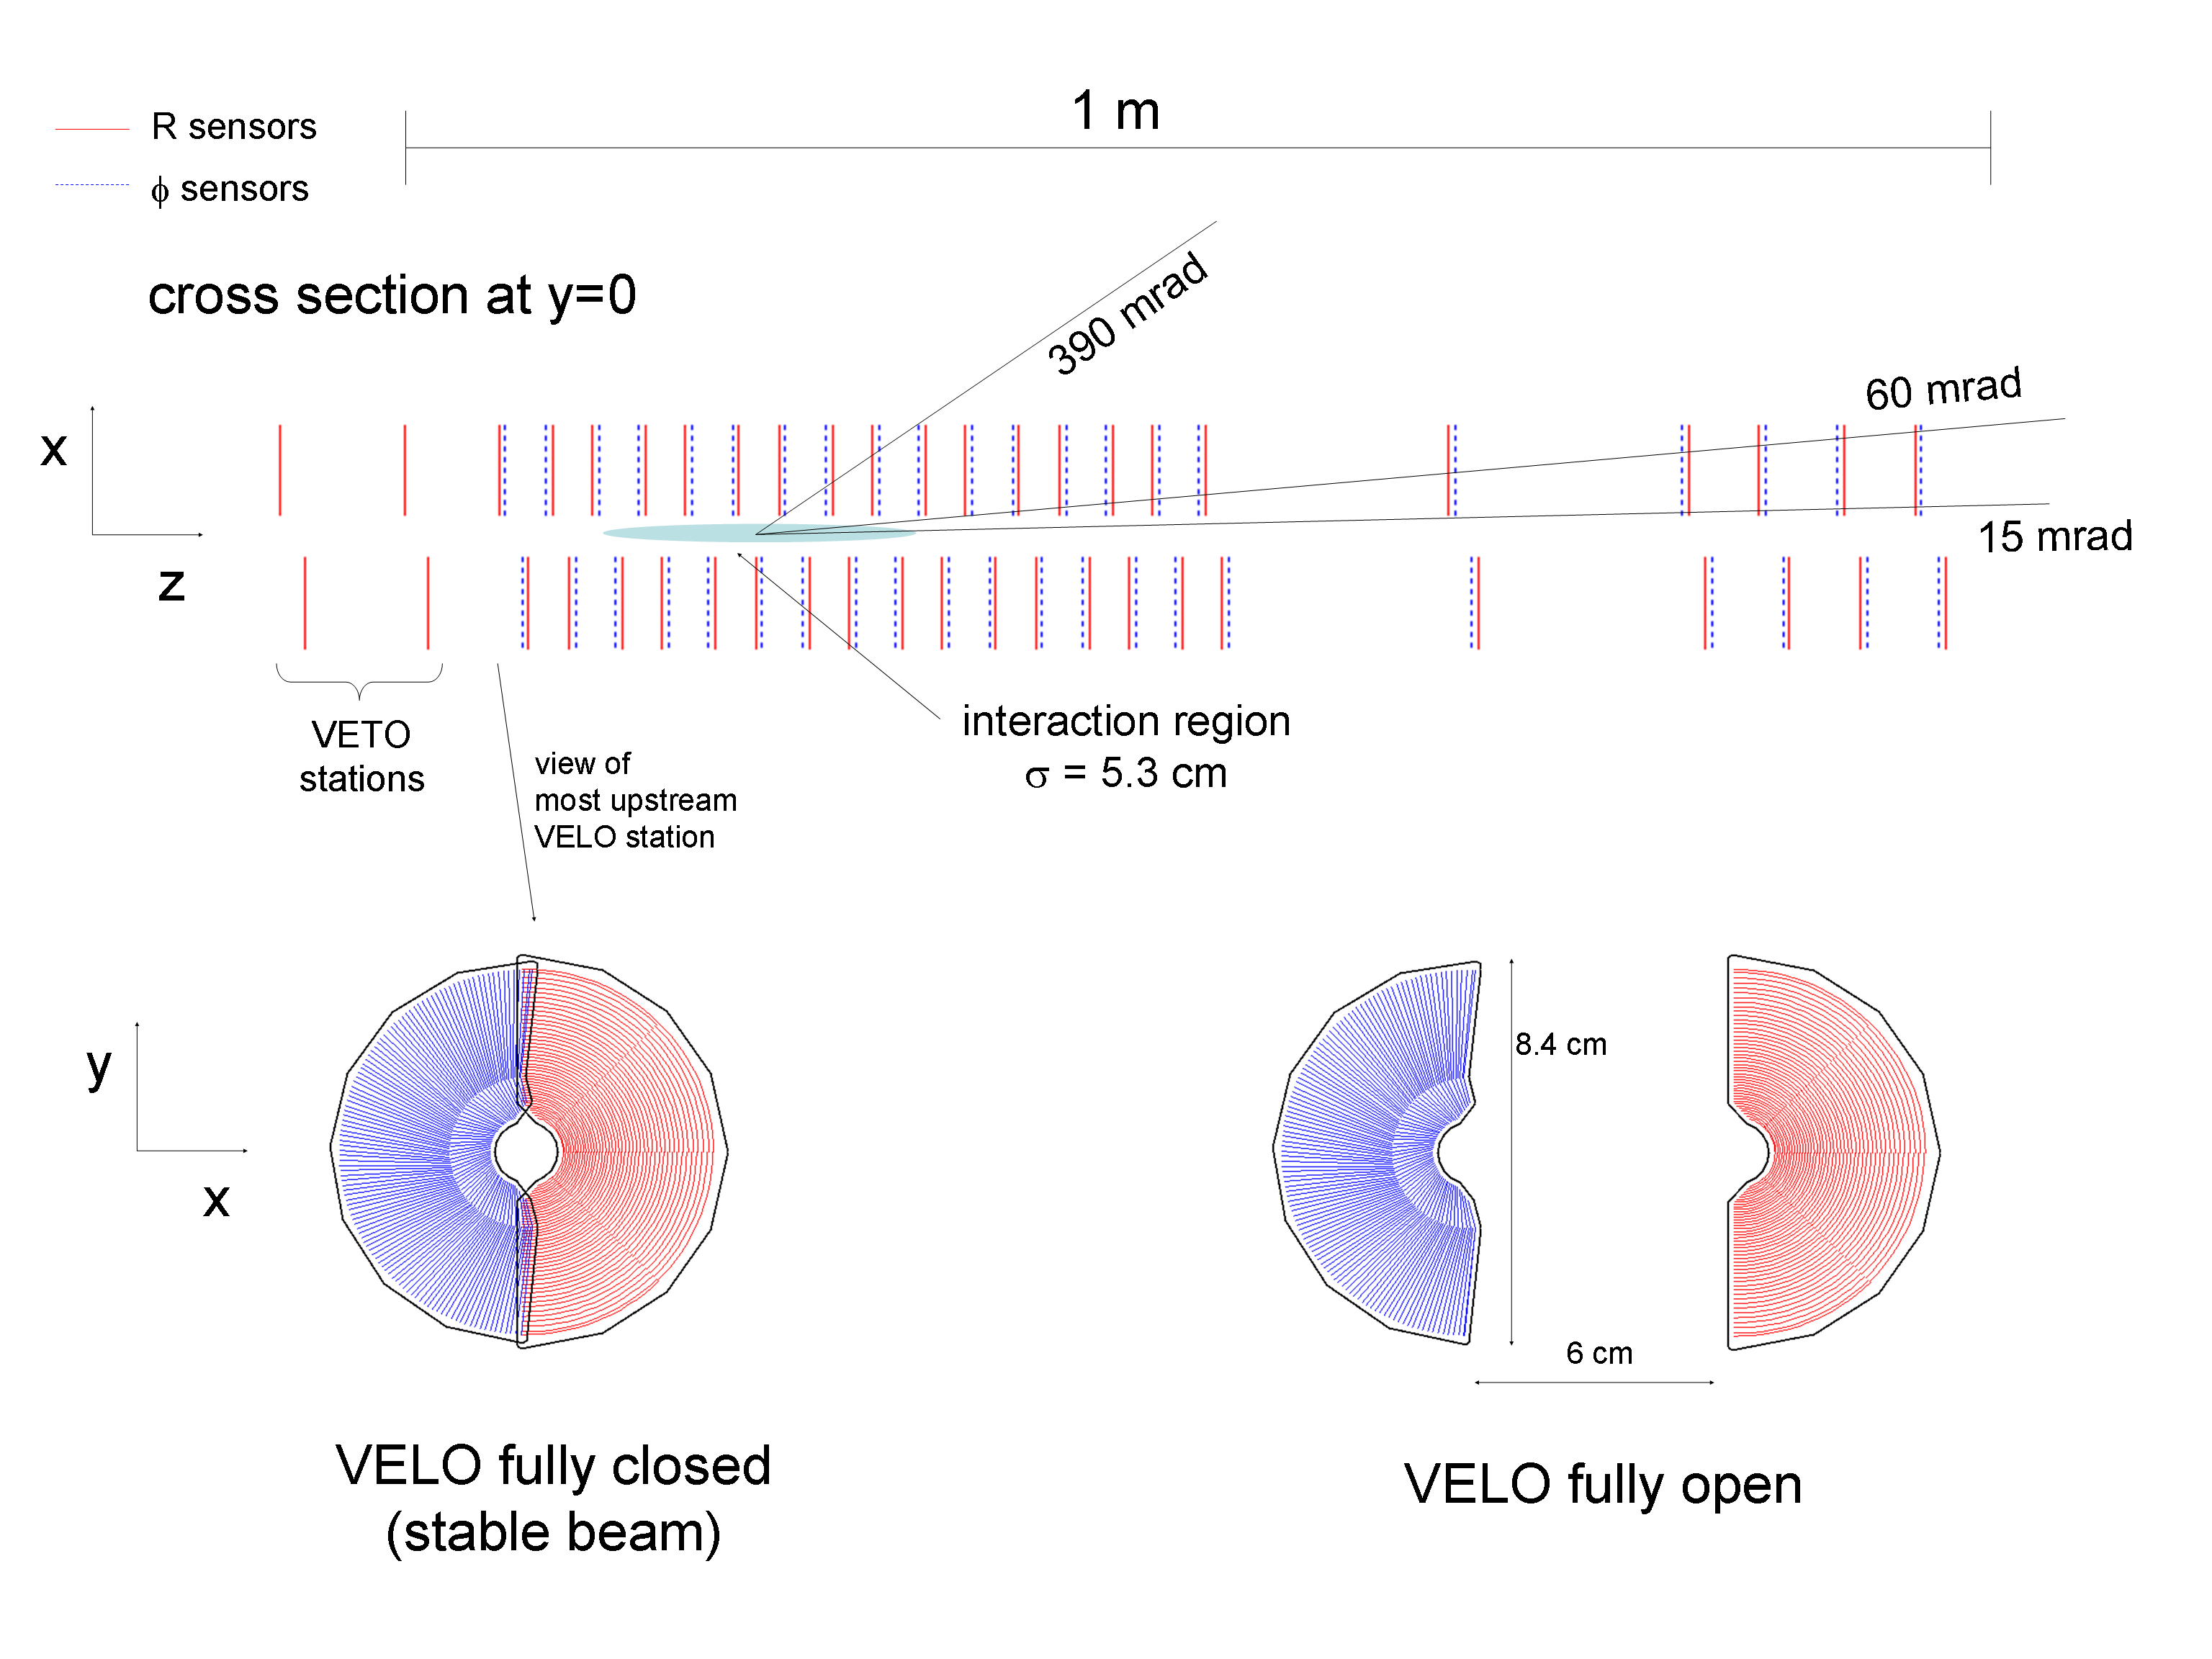
\includegraphics[width=0.8\textwidth]{VELO_Overview}	
	\caption{Cross section in the $(x,z)$ plane of the VELO silicon sensors, at $y=0$, with the detector in the fully closed position. 
             The front face of the first modules is also illustrated in both the closed and open positions. 
             The two pile-up veto stations are located upstream of the VELO sensors.
             Figure and caption taken from \cite{detector}.}
	\label{fig:VELO_Overview}
\end{figure}
With this setup the VELO reaches a track finding efficiency above 98\%. 
Its resolution on vertices is 13\mum in the transverse plane and 71\mum along the beam axis for vertices with 25 tracks. 
The resolution on the impact parameter is smaller than 35\mum for particles with a transverse momentum larger than 1\gev \cite{detector, VELO_TDR, VELO_Performance}.

\subsection{Silicon Tracker (ST)}
The Silicon Tracker (ST) uses silicon microstrip detectors with a strip pitch of about 200\mum.
It comprises two detectors: the Tracker Truciensis (TT) and the Inner Tracker (IT).
The Tracker Turicencis or formerly the Trigger Tracker is located in front of the entrance of the \lhcb magnet. 
It is used for sevaral tasks:
\begin{itemize}
    \item deliver transverse momentum information for Level-1 trigger,
    \item reconstruct trajectories of long-lived neutral particles decaying outside the VELO
    \item reconstruct low-momenta particles bent out by the magnet before reaching the station T1-T3.
\end{itemize}
The TT consists of one station made of four planes along the beam axis. 
The first and the fourth layer have vertical readout strips ($x$-layer), while the second and third are rotated by an angle $\pm 5\degrees$ to get a high resolution in the bending plane and additional information in $y$-direction.
Between the $u$ and $v$ layer there is a gap of around 30\cm. 
Figure \ref{fig:TT_layers} shows schematically the layout of the TT.
\begin{figure}[hptb]
    \centering
	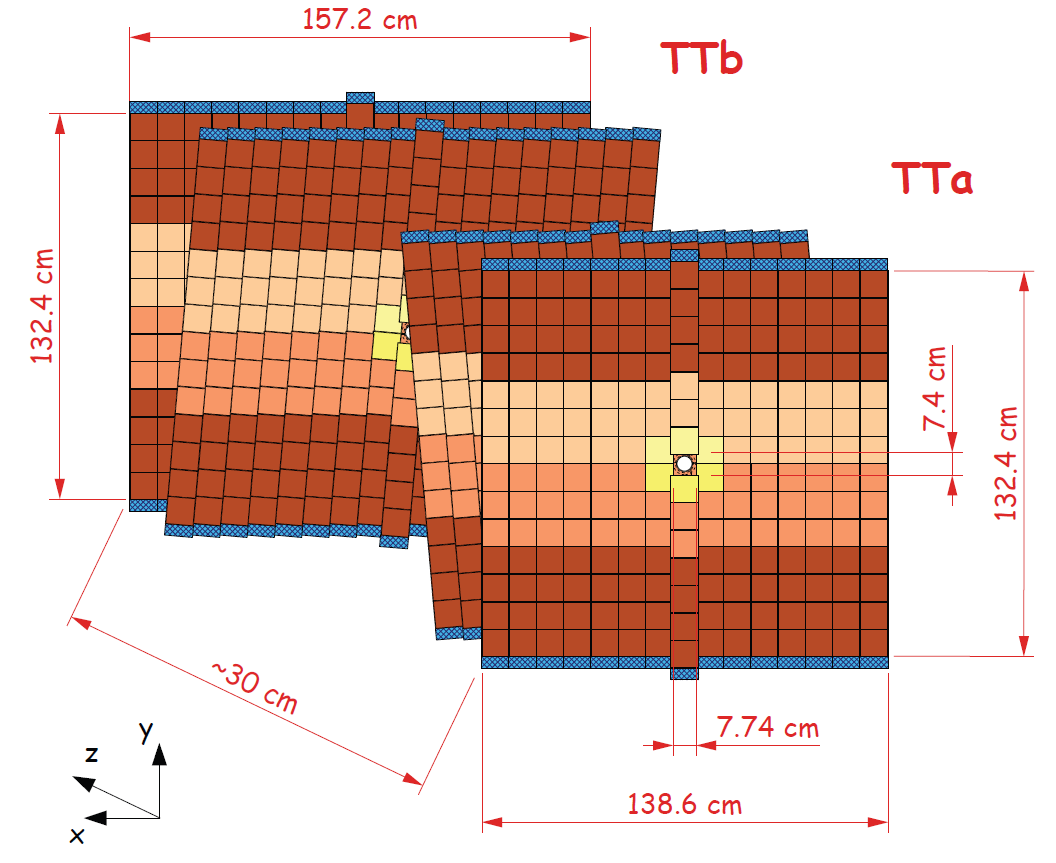
\includegraphics[width=0.8\textwidth]{TT_layers}	
	\caption{Layout of the Tracker Turicensis (TT). 
             Figure taken from \cite{ST_Performance}.}
	\label{fig:TT_layers}
\end{figure}
The Inner Tracker uses the same technology as the TT as already mentioned. 
It builds the inner part of the three tracking stations T1-T3 (see Figure \ref{fig:detector}), which are located downstream the magnet.
Each station consists of four boxes as shown in figure \ref{fig:IT_layer}.
In each box there are again 4 layers, two vertical and two stereo, analogously to the TT. 
Though the IT only covers 1.3\% of the geometrical acceptance, 20\% of the track are passing it \cite{detector, ST_Performance}.
\begin{figure}[hptb]
    \centering
	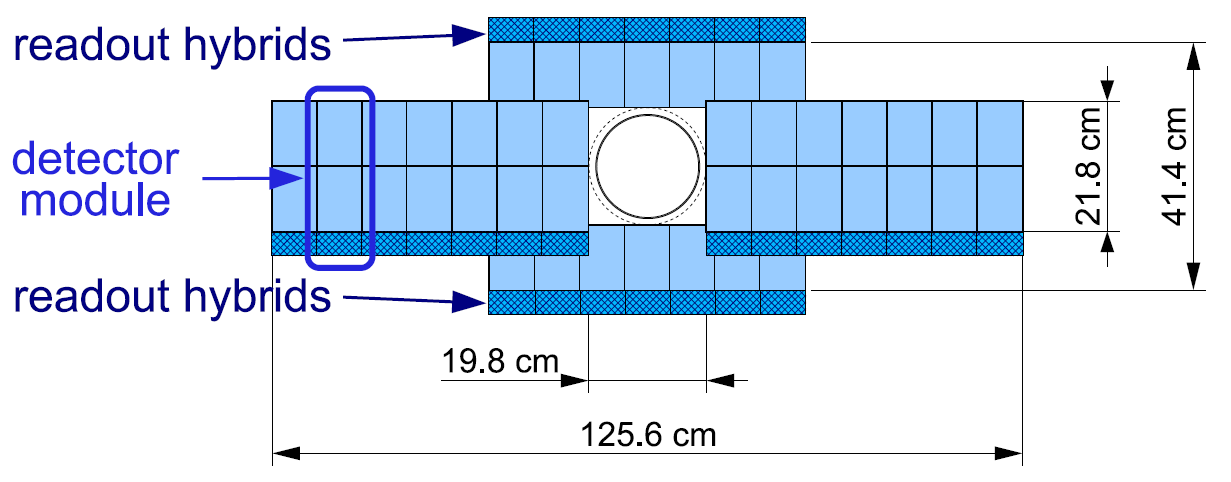
\includegraphics[width=0.8\textwidth]{IT_layer}	
	\caption{Layout of a $x$ detection layer in the second Inner Tracker (IT) station. 
             Figure taken from \cite{detector}.}
	\label{fig:IT_layer}
\end{figure}

\subsection{Outer Tracker (OT)}
The Outer Tracker builds the outer part of the Tracking stations T1-T3 downstream the magnet.
It is a gaseous straw tube detector covering an area of approximately $5 \times 6 \ma$ with 12 double layers of straw tubes.
The straw tubes are filled with a gas mixture of argon (70\%), carbon dioxide (28.5\%) and oxygen (1.5\%).
This guarantees a drift time of less than 50\ns enabling to distinguish consecutive proton bunch collisions.
Again the three stations consist of 4 layers each in $x-u-v-x$ geometry.
The spatial resolution is 200\mum along the $x$ axis.
On the one hand this is worse than the spatial resolution of the IT with 50\mum, but on the other hand the angular coverage is much higher \cite{OT_Performance}.

\subsection{Track classification}


% ================================
% SECTION: Particle identification
% ================================
\section{Particle identification}

\subsection{Ring Imaging Cherenkoy Detector (RICH)}

\subsection{Calorimeter system}

\subsection{Muon chambers}

% ===========================
% SECTION: Trigger
% ===========================
\section{Trigger}

\subsection{L0-Trigger}

\subsection{High Level Trigger (HLT)}
